% !TeX spellcheck = en_US

\chapter{Related Work}
This chapter elaborates on the base technologies necessary to understand the following chapters.


\section{Geographic Information System (GIS)}
GIS contains of numerous technologies to store, manipulate and analyze geographical data. 


\subsection{Coordinate Reference System (CRS)}
In comparison to normal image data, GIS data is always geo-referenced. This is achieved by specific geo-aware formats that encode the spatial position into the file. Reading and writing GIS requires specialized software.\\
When displaying GIS, it is almost always necessary to project the round shape of earth onto a plane. This projection can be done in numerous ways called \enquote{spatial reference system} (SRS) or  \enquote{coordinate reference system} CRS. Depending on the area of earth, different projections result in optimal results (see figure \ref{fig:mercator}).
\begin{figure}[H]
	\centering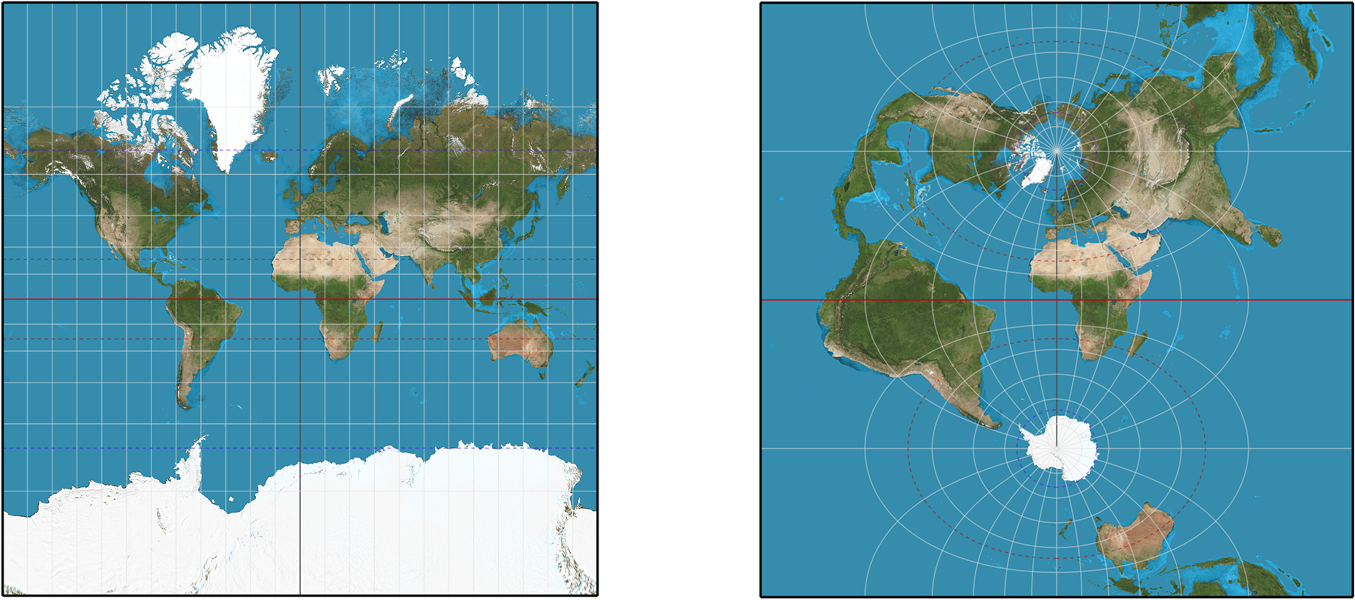
\includegraphics[width=1\textwidth]{res/Mercator}
	\caption{Normal and transverse Mercator projection by Peter Mercator. \url{https://commons.wikimedia.org/w/index.php?curid=9910866}}
	\label{fig:mercator}
\end{figure}
For viewing the whole world, the \enquote{World Geodetic System 1984} (WGS 84) is the most common CRS. It also exists as an \enquote{European Petroleum Survey Group}  (EPSG) standard. EPSG:4326 is the most recent version of this projection. It is used by the Global Positioning System (GPS), as well as map applications like OpenStreetMap (OSM) and Google Maps.


\subsection{File Types}
GIS files exist in two different types. vector and raster.

\subsubsection{Raster Data}
 Raster data consists of a grid that is filled with color values. The advantage of raster data is that it can store any kind of GIS. the disadvantages are big files and the lack of scalability.

\subsubsection{Vector Data}
Raster GIS on the other hand has a much smaller file size, but is limited in its capabilities. It can store points, polylines and polygons, which makes it a good match for displaying hot-spots, borders, contour lines, etc.



\section{Mono}
Open C\# implementation for Linux and OSX.



\section{.NET Core}
Microsoft bought Xamarin, which mostly developed Mono and is creating it's new C\# with build in multi-platform support.